%! app: Regular Languages, Context-free Languages
%! outcome: Formal definition of automata, Informal definition of automata, Nondeterminism, Classify language, Find example languages
    
    
For the PDA state diagrams below, $\Sigma = \{0,1\}$.


\begin{center}
\begin{tabular}{c c}
Mathematical description of language & State diagram of PDA recognizing language\\
\hline
& $\Gamma = \{ \$, \#\}$ \hspace{2.3in} \\
& \\
& 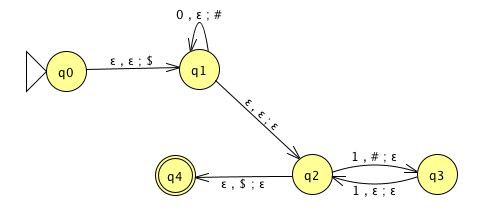
\includegraphics[width=3.5in]{../../resources/machines/Lect10PDA1.png}\\
& \\
& \\
\hline
& $\Gamma = \{ {@}, 1\}$ \hspace{2.3in} \\
& \\
& 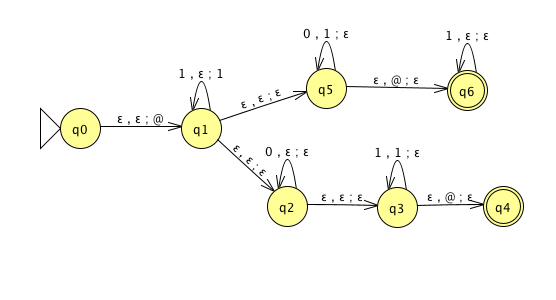
\includegraphics[width=3.5in]{../../resources/machines/Lect10PDA2.png}\\
& \\
& \\
\hline
& \\
& \\
& \\
$\{ 0^i 1^j 0^k \mid i,j,k \geq 0 \}$ & \\
& \\
& \\
\end{tabular}
\end{center}

\newpage
{\it Big picture}: PDAs were motivated by wanting to add some memory of unbounded size to NFA. How 
do we accomplish a similar enhancement of regular expressions to get a syntactic model that is 
more expressive?

DFA, NFA, PDA: Machines process one input string at a time; the computation of a machine on its input string 
reads the input from left to right.

Regular expressions: Syntactic descriptions of all strings that match a particular pattern; the language 
described by a regular expression is built up recursively according to the expression's syntax

{\bf Context-free grammars}: Rules to produce one string at a time, adding characters from the middle, beginning, 
or end of the final string as the derivation proceeds.


\begin{center}
  \hspace{-0.25in}\begin{tabular}{|p{2in}cp{4in}|}
  \hline 
  Term & Typical symbol & Definition \\
  \hline\hline
  {\bf Context-free grammar} (CFG) & $G$ & $G = (V, \Sigma, R, S)$ \\
  {\bf Variables}& $V$ & Finite  set of symbols that represent phases in production pattern\\
  {\bf Terminals} & $\Sigma$ & Alphabet of symbols of strings generated  by CFG \\
  & & $V \cap \Sigma = \emptyset$ \\
  {\bf Rules}& $R$ & Each rule is  $A \to u$ with $A \in V$ and $u  \in (V  \cup \Sigma)^*$\\
  Start variable&  $S$  & Usually  on LHS of first / topmost rule \\
  {\bf Derivation} & & Sequence  of substitutions in a  CFG \\
  & $S \implies \cdots \implies w$ & Start with start variable, apply one rule to one occurrence of a variable at a time\\
  {\bf Language} generated by the CFG $G$ & $L(G)$ &$\{  w \in \Sigma^* \mid \text{there is  derivation in $G$ that ends
  in $w$} \} = \{  w \in \Sigma^* \mid S \implies^* w \}$\\
  {\bf Context-free language} & & A language that is the language generated by some CFG\\
  \hline
  Sipser pages 102-103 & &\\
  \hline
  \end{tabular}
  \end{center}
  
{\bf Examples of context-free grammars, derivations in those grammars, and the languages generated by those grammars}
  
$G_1 =  (\{S\}, \{0\}, R, S)$ with rules
  \begin{align*}
    &S \to 0S\\
    &S \to 0\\
  \end{align*}
  In  $L(G_1)$ \ldots 
  
  \vspace{110pt}
  
  Not in $L(G_1)$ \ldots 

  \vspace{110pt}

\newpage
  $G_2 =  (\{S\}, \{0,1\}, R, S)$
  \[
  S \to 0S \mid 1S \mid \varepsilon
  \]
  In  $L(G_2)$ \ldots 
  
  \vspace{110pt}
  
  Not in $L(G_2)$ \ldots 

  \vspace{110pt}

  $(\{S, T\}, \{0, 1\}, R, S)$ with  rules
  \begin{align*}
  &S \to T1T1T1T \\
  &T \to  0T \mid 1T \mid \varepsilon
  \end{align*}

  In  $L(G_3)$ \ldots 
  
  \vspace{110pt}
  
  Not in $L(G_3)$ \ldots 

  \vspace{110pt}

\newpage
  $G_4 =  (\{A, B\}, \{0, 1\}, R, A)$ with rules
  \[
    A \to 0A0 \mid  0A1 \mid 1A0  \mid 1A1 \mid  1
  \]
  In  $L(G_4)$ \ldots 
  
  \vspace{110pt}
  
  Not in $L(G_4)$ \ldots 

  \vspace{110pt}

  
{\it Extra practice}: Is there a CFG $G$ with $L(G) = \emptyset$?
